\section{Use Case model} \label{sec:UseCaseModel}
%%%%%%%%%%%%%%%%%%%%%%%%%%%%
Model případu užití popisuje funkcionalitu systému z pohledu uživatele. 

Model byl rozdělen podle etap vývoje zmíněných v sekci \ref{subsec:strategie_naplnění_vize}.
Do první etapy patří aktér \emph{Administrátor} a případy užití UC1 až UC6.

Součástí druhé etapy je aktér \emph{Zákazník} a jeho případy užití: UC7, UC8, UC9. 

Diagram modelu je vidět na obrázku \ref{fig:Use_case_diagram}, prvky druhé etapy jsou označeny zelenou barvou.
%%%%%%%%%%%%%%%%%%%%%%%%%%%%
\subsection{Aktéři}
\begin{description}
    \item [Actor 1:] Administrátor.
    \begin{itemize}
        \item Administrátor je osoba zodpovědná za administrativu pneuservisu. (Majitel pneuservisu)
    \end{itemize}
    \item [Actor 2:] Zákazník.
    \begin{itemize}
        \item Zákazník je koncový uživatel služeb pneuservisu. 
    \end{itemize}
\end{description}
%%%%%%%%%%%%%%%%%%%%%%%%%%%%
\subsection{Use case}
\begin{description}
    \item [UC1:] Přehled informací o zákazníkovi.
    \begin{itemize}
        \item Administrátor si může otevřít zákaznickou kartu s informacemi o zákazníkovi, jeho vozidlech, discích, pneumatikách a objednaných službách.
    \end{itemize}
    \item [UC2:] Registrace nového zákazníka. 
    \begin{itemize}
        \item Administrátor registruje nového zákazníka do systému. Ukládá identifikační údaje o zákazníkovi.
    \end{itemize}
    %\pagebreak
    \item [UC3:] Registrace automobilu zákazníka. 
    \begin{itemize}
        \item Administrátor registruje automobil. Ukládá identifikační údaje o automobilu. 
    \end{itemize}
    \item [UC4:] Registrace disků a pneumatik.
    \begin{itemize}
        \item Administrátor registruje disky a pneumatiky. Ukládá jejich identifikační údaje.
    \end{itemize}
    \item [UC5:] Rezervace zákazníka na přezutí a objednání služeb.
    \begin{itemize}
        \item Administrátor v systému rezervuje zákazníka na přezutí a objednává další služby. 
    \end{itemize}
    \item [UC6:] Automatické rozesílání e-mailů.
    \begin{itemize}
        \item Administrátor má možnost nastavit pravidelné emaily upozorňující na blížící se sezónu nebo blížící se termín přezutí. 
    \end{itemize}
    \item [UC7:] Registrace.
    \begin{itemize}
        \item Koncový zákazník se registruje na webových stránkách. 
    \end{itemize}
    \item [UC8:] Registrace vlastního automobilu.
    \begin{itemize}
        \item Koncový zákazník registruje svůj automobil. 
    \end{itemize}
    \item [UC9:] Rezervace na přezutí a objednání služeb.
    \begin{itemize}
        \item Koncový zákazník se rezervuje na přezutí a objednává si doplňkové služby.
    \end{itemize}
\end{description}
\begin{figure}[h!]
    \centering
    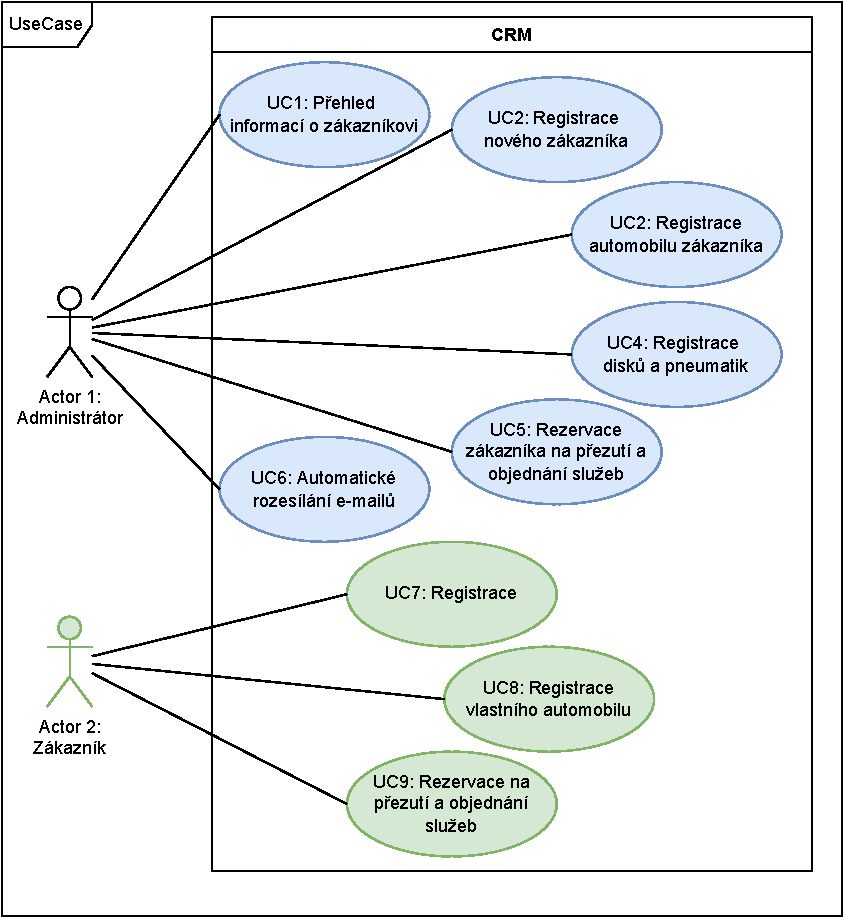
\includegraphics[width=0.75\textwidth]{assets/6_návrh/CRM Usecase Diagram.drawio.pdf}
    \caption{Use case diagram.}
    \label{fig:Use_case_diagram}
\end{figure}
\FloatBarrier
